% !TEX program = xelatex

%%%%%%%%%%%%%%%%%%%%%%%%%%%%%%%%%%%%%%%%%
% Thin Sectioned Essay
% LaTeX Template
% Version 1.0 (3/8/13)
%
% This template has been downloaded from:
% http://www.LaTeXTemplates.com
%
% Original Author:
% Nicolas Diaz (nsdiaz@uc.cl) with extensive modifications by:
% Vel (vel@latextemplates.com)
%
% License:
% CC BY-NC-SA 3.0 (http://creativecommons.org/licenses/by-nc-sa/3.0/)
%
%%%%%%%%%%%%%%%%%%%%%%%%%%%%%%%%%%%%%%%%%

%----------------------------------------------------------------------------------------
%	PACKAGES AND OTHER DOCUMENT CONFIGURATIONS
%----------------------------------------------------------------------------------------

\documentclass[a4paper, 11pt]{article} % Font size (can be 10pt, 11pt or 12pt) and paper size (remove a4paper for US letter paper)
\usepackage[table,xcdraw]{xcolor}\usepackage{cite}
\usepackage{fontspec}
\definecolor{keycolor}{RGB}{172, 42, 42}
\definecolor{mbleu}{RGB}{64,96,127}
\definecolor{vimvert}{RGB}{46, 139, 87}
\usepackage{hyperref}
\usepackage{placeins} 
% \setmainfont{Avenir Next}
% \setsansfont{Avenir Next}

\usepackage{xeCJK}

\usepackage{geometry}
\geometry{left=2.54cm, top=2.54cm, right=2.54cm, bottom=2.54cm}
\usepackage{subcaption}
\usepackage{tikz}
\usetikzlibrary{tikzmark}
\usepackage{listings}
\usepackage{color}
\usepackage{forest}
\usepackage{float}
\usepackage{makecell}
\usepackage[binary-units]{siunitx}
\usepackage{enumitem}

\lstset{
basicstyle=\small,%
escapeinside=``,%
keywordstyle=\color{blue} \bfseries,% \underbar,%
identifierstyle={},%
commentstyle=\color{blue},%
stringstyle=\ttfamily,%
%labelstyle=\tiny,%
extendedchars=false,%
linewidth=\textwidth,%
numbers=left,%
numberstyle=\tiny \color{blue},%
frame=trbl%
}
 
\newcounter{code}
\lstnewenvironment{code}[3][C++]%
  {%
    \renewcommand\lstlistingname{代码}
    \lstset{% frame=tb,
    language=#1,
    caption=#2,
    label=#3
    }
  }{}

% \usepackage{fancyhdr}
% \usepackage{lastpage}
% \pagestyle{fancy}
% \fancyhf{}
% \fancyfoot[R]{第 \thepage 页,共 \pageref{LastPage} 页}
% % \fancyfoot[C]{\thepage/\pageref{LastPage}}
% \renewcommand{\headrulewidth}{0pt} 
% \renewcommand{\footrulewidth}{0.4pt} 
\renewcommand{\lstlistingname}{Code} % Listing->Code

% \usepackage[protrusion=true,expansion=true]{microtype} % Better typography
\usepackage{graphicx} % Required for including pictures
\usepackage{wrapfig} % Allows in-line images
\usepackage{newfloat}
\usepackage{amsmath}
\usepackage{multirow}

\usepackage{mathpazo} % Use the Palatino font
\usepackage[T1]{fontenc} % Required for accented characters
\linespread{1.2} % Change line spacing here, Palatino benefits from a slight increase by default
% \setlength{\parskip}{0.2em}

\usepackage{indentfirst}
\setlength{\parindent}{2em}

\makeatletter
\renewcommand\@biblabel[1]{\textbf{#1.}} % Change the square brackets for each bibliography item from '[1]' to '1.'
\renewcommand{\@listI}{\itemsep=0pt} % Reduce the space between items in the itemize and enumerate environments and the bibliography

\renewcommand{\maketitle}{ % Customize the title - do not edit title and author name here, see the TITLE block below
\begin{center} % Right align
{\LARGE\@title} % Increase the font size of the title

\large{\@subtitle}

\vspace{1em} % Some vertical space between the title and author name

{\large\@author} % Author name
% \\\@date % Date

% \vspace{1.5em} % Some vertical space between the author block and abstract
\end{center}
}

\renewcommand{\figurename}{图}
\renewcommand{\tablename}{表}

%----------------------------------------------------------------------------------------
%	TITLE
%----------------------------------------------------------------------------------------

\title{\textbf{操作系统实验项目}\\ % Title
} % Subtitle
\newcommand\@subtitle{实现系统调用}

\author{郑戈涵\quad 17338233\quad 931252924@qq.com} % Institution

\date{2020年5月3日} % Date


%----------------------------------------------------------------------------------------

\begin{document}

\maketitle % Print the title section

%----------------------------------------------------------------------------------------
%	ABSTRACT AND KEYWORDS
%----------------------------------------------------------------------------------------

\renewcommand{\abstractname}{摘要} % Uncomment to change the name of the abstract to something else

\begin{abstract}
  本次实验共完成三个任务:实现中断保护,完成软中断程序编写,生成自己的COM程序
\end{abstract}

% \hspace*{3,6mm}\texttt{Keywords:} lorem , ipsum , dolor , sit amet , lectus % Keywords

\vspace{1em} % Some vertical space between the abstract and first section

\setcounter{tocdepth}{2}
\renewcommand{\contentsname}{目录}
\tableofcontents

% \vspace{2em} % Some vertical space between the abstract and first section

\pagebreak

\section{实验目的}

% 问题、方法、实验目的、意义
\begin{enumerate}
  \item 学习多道程序与CPU分时技术
  \item 掌握操作系统内核的二态进程模型设计与实现方法
  \item 掌握进程表示方法
  \item 掌握时间片轮转调度的实现
\end{enumerate}


\section{实验要求}

\begin{enumerate}
  \item 了解操作系统内核的二态进程模型
  \item 扩展实验五的的内核程序,增加一条命令可同时创建多个进程分时运行,增加进程控制块和进程表数据结构。
  \item 修改时钟中断处理程序,调用时间片轮转调度算法。
  \item 设计实现时间片轮转调度算法,每次时钟中断,就切换进程,实现进程轮流运行。
  \item 修改save()和restart()两个汇编过程,利用进程控制块保存当前被中断进程的现场,并从进程控制块恢复下一个进程的现场。
\end{enumerate}

\section{实验内容}

% 输入、输出形式,使用的数据结构,算法的描述,算法正确性说明,算法分析,算法实现所需变量,没有代码
\subsection{设计PCB数据结构}

修改实验5的内核代码,定义进程控制块PCB类型,包括进程号、程序名、进程内存地址信息、CPU寄存器保存区、进程状态等必要数据项,再定义一个PCB数组,最大进程数为10个。

\subsection{设计多进程命令}

扩展实验五的的内核程序,增加一条命令可同时执行多个用户程序,内核加载这些程序,创建多个进程,再实现分时运行

\subsection{修改时钟中断处理程序}

修改时钟中断处理程序,保留无敌风火轮显示,而且增加调用进程调度过程

\section{实验原理}
\subsection{两进程模型}
在任何时刻,一个进程要么正在执行,要么未执行,因而可以构建最简单的模型。进程可处于以下两种状态之一:运行态或未运行态,
如图3.5(a)所示。操作系统创建一个新进程时,它将该进程以未运行态加入系统,操作系统知道这个进程的存在,并正在等待执行机会。时而不时地,
当前正在运行的进程会被中断,此时操作系统中的分派器部分将选择一个新进程运行。前一个进程从运行态转换为未运行态,后一个进程则转换为运行态。\cite{gityuan2016}

\subsubsection{进程的创建}
进程的创建将一个新进程添加到正被管理的进程集时,操作系统需要建立用于管理该进程的数据结构(见33节),并在内存中给它分配地址空间,这些行为构成了一个新进程的创建过程。
触发进程创建的事件通常有4个,如表3.1所示。在批处理环境中,响应作业提交时会创建进程;在交互环境中,当新用户试图登录时会创建进程。不论哪种情况,操作系统都负责新进程的创建工作。
操作系统也可能会代表应用程序创建进程。例如,如果用户请求打印一个文件,则操作系统可以创建一个管理打印的进程,进而使请求进程可以继续执行,与完成打印任务的时间无关。
\subsubsection{进程终止}
表\ref{processhalt}概括了进程终止的典型原因。任何一个计算机系统都必须为进程提供表示其完成的方法,批处理作业中应包含一个Halt指令或其他操作系统显式服务调用来终止。
在前一种情况下,Halt指令将产生一个中断,警告操作系统一个进程己经完成。对交互式应用程序,用户的行为将指出何时进程完成。例如,在分时系统中,
当用户退出系统或关闭自己的终端时,该用户的进程将被终止。在个人计算机或工作站中,用户可以结束一个应用程序(如字处理或电子表格)。所有这些行为最终将导致给操作系统发出一个服务请求,
以终止发出请求的进程。此外,很多错误和故障条件会导致进程终止。表32列出了一些最常见的识别条件最后,在有些操作系统中,进程可被创建它的进程终止,或在父进程终止时而终止。

% Please add the following required packages to your document preamble:
% \usepackage[table,xcdraw]{xcolor}
% If you use beamer only pass "xcolor=table" option, i.e. \documentclass[xcolor=table]{beamer}
\begin{table}[]
  \caption{导致进程终止的原因}
  \label{tab:process_halt}
  \begin{tabular}{
  >{\columncolor[HTML]{FFFFFF}}l 
  >{\columncolor[HTML]{FFFFFF}}l }
  事件         & 说明                                                                                                                                                  \\
  正常完成       & {\color[HTML]{333333} 进程自行执行一个操作系统服务调用,表示它己经结束运行}                                                                                                   \\
  超过时限       & {\color[HTML]{333333} \begin{tabular}[c]{@{}l@{}}进程运行时间超过规定的时限。可以测量多种类型的时间,包括总运行时间\\ (“挂钟时间”)、花费在执行上的时间,以及对于交互进程从上一次\\ 用户输入到当前时刻的时间总量\end{tabular}} \\
  无可用内存      & {\color[HTML]{333333} 系统无法满足进程需要的内存空间}                                                                                                              \\
  超出范围       & {\color[HTML]{333333} 进程试图访问不允许访问的内存单元}                                                                                                             \\
  保护错误       & \begin{tabular}[c]{@{}l@{}}进程试图使用不允许使用的资源或文件,或试图以一种不正确的方式使用,\\ 如往只读文件中写\end{tabular}                                                                \\
  算术错误       & 进程试图进行被禁止的计算,如除以零或存储大于硬件可以接纳的数字                                                                                                                     \\
  时间超出       & 进程等待某一事件发生的时间超过了规定的最大值                                                                                                                              \\
  I/O失败      & \begin{tabular}[c]{@{}l@{}}在输入或输出期间发生错误,如找不到文件、在超过规定的最多努力次数后仍然\\ 读/写失败(如遇到磁带上的一个坏区时)或无效操作(如从行式打印机中读)\end{tabular}                                   \\
  无效指令       & 进程试图执行一个不存在的指令(通常是由于转移到了数据区并企图执行数据)                                                                                                                 \\
  特权指令       & 进程试图使用为操作系统保留的指令                                                                                                                                    \\
  数据误用       & 错误类型或未初始化的一块数据                                                                                                                                      \\
  操作员或操作系统干涉 & 由于某些原因,操作员或操作系统终止进程(如出现死锁时)                                                                                                                         \\
  父进程终止      & 当一个父进程终止时,操作系统可能会自动终止该进程的所有子进程                                                                                                                      \\
  父进程请求      & 父进程通常具有终止其任何子进程的权力                                                                                                                                 
  \end{tabular}
  \end{table}
\section{实验过程}

本次实验流程如下:
\begin{enumerate}
  \item 修改用户程序的执行方式
  \item 设计PCB数据结构
  \item 修改save和restart过程
  \item 修改时钟中断程序
  \item 修改shell的运行逻辑(增加多进程处理)
\end{enumerate}

\subsection{修改用户程序的执行方式}
在上次的实验中,我已经修改了执行程序为如下方式:
\begin{enumerate}
  \item 将用户程序所在的镜像加载进内存中
  \item 将用户程序的地址信息放进一个内存块中
  \item 预先埋好用户程序返回所需的信息
  \item 利用上一步的内存块,用远跳转(jmp far)跳入用户程序第一条指令的地址
  \item 用户程序执行结束后用20号中断程序转去执行后处理程序(恢复内核段寄存器等)
  \item 返回内核shell
\end{enumerate}

这次实验中,由于需要增加一种运行程序的方式,原来的执行方式需要分开,即分为加载程序和运行程序两个过程,什么时候执行由内核处理。
\subsubsection{加载模块}
由于加载完成后,不应该限制用何种方式运行程序。因此加载过程需要将所有运行程序前的准备都完成。具体有三点:
\begin{enumerate}
  \item 将用户程序所在的镜像通过13号中断加载进内存中
  \item 在用户程序头放入int 20h
  \item 在栈中预先埋好地址用于几次返回
\end{enumerate}
在上次的代码的基础上,首先将int 13h之前的语句分出。由于使用用户栈需要修改ss,在ss修改为用户程序所在段后,就不能使用内核栈了,因此我使用内核的内存来保存需要的信息(内核的sp等)
其中还需要使用es等段寄存器用于修改用户程序信息,返回前需要恢复。代码如下:

\begin{lstlisting}[language={[x86masm]Assembler},label=loadUsrProgram,caption=loadUsrProgram]
  loadUsrProgram:    
  pusha
  push es       
  mov bp, sp
  mov bx, [bp+22]        ; 程序信息结构体指针
  mov ax, [bx+20]        ; 存放数据的段地址
  mov es, ax             ; 用es才能跨段读取,es:bx是读入的数据所在内存地址
  mov ah,2               ; 功能号
  mov al,[bx+12]         ; 扇区数
  mov dl,0               ; 驱动器号; 软盘为0,硬盘和U盘为80H
  mov dh, [bx+4]         ; 磁头号; 起始编号为0
  mov ch, [bx]           ; 柱面号; 起始编号为0
  mov cl, [bx+8]         ; 起始扇区号 ; 起始编号为1
  mov bx, [bx+16]        ; 存放数据的内存偏移地址
  int 13H                ; 调用读磁盘BIOS的13h功能
  mov word[cs:savesp],sp ; 保存当前的栈顶,用于返回后恢复
  mov sp,0xff00          ; 设置用户程序的栈顶
  mov bx, es
  mov ss, bx             ; 设置现在的栈段和es一致(以后push和pop就会操作用户程序的栈)
  mov ax,[cs:codeOfInt20]; 用ax保存int 20这个语句
  mov [es:0],ax          ; 在es:0(用户程序所在段首)放置int 20
  push cs                ; 
  push afterRun          ; 将cs ip先后压栈,返回时可以远返回retf
  push dword 0           ; 压栈0,用户程序如果使用ret就会触发ip=0的操作,开始执行从es:0开始的语句
  mov bx, cs
  mov ss, bx
  mov sp,[cs:savesp]
  pop es
  popa
  retf
\end{lstlisting}

\subsubsection{运行模块}
运行模块是用于批处理或者执行单个程序的,将各个段寄存器和栈寄存器设置好,压入地址并远返回即可转到用户程序的100h处开始执行。代码如下:
\begin{lstlisting}[language={[x86masm]Assembler},label=runUsrProgram,caption=runUsrProgram]
  runUsrProgram:
  pusha
  mov bp, sp
  mov bx, [bp+20]        ; 程序信息结构体指针
  mov ax, cs
  mov gs, ax
  mov word[gs:savesp],sp ; 保存当前的栈顶,用于返回后恢复
  mov ax,0xff00          ; 用户程序的栈顶为0xff00
  mov sp, ax             ; 设置用户程序的栈顶
  sub sp, 8
  mov bx, [bx+20]
  mov es, bx             ; 用es才能跨段读取,es:bx是读入的数据所在内存地址
  mov ds, bx             ; 设置用户程序的数据段和es一致
  mov ss, bx             ; 设置现在的栈段和es一致(以后push和pop就会操作用户程序的栈)
  push bx
  push 0x100
  retf                   ;远返回至bx:100
\end{lstlisting}


\subsection{设计PCB数据结构}

\subsubsection{PCB结构体设计}
上次实验中已经设计了寄存器映像,这次只需要加上pid和state就可以,pid是进程号,state用于记录该进程的状态,目前只有新进程、就绪和运行三种是可用的,新进程意味着该PCB未被使用。代码如下:
\begin{lstlisting}[language={c},label=RegisterImage,caption=struct RegisterImage]
  enum PCB_STATE {P_NEW, P_READY, P_RUNNING, P_BLOCKED, P_EXIT};
  
  typedef struct RegisterImage{
    uint16_t ax;     // 0
    uint16_t cx;     // 2
    uint16_t dx;     // 4
    uint16_t bx;     // 6
    uint16_t sp;     // 8
    uint16_t bp;     // 10
    uint16_t si;     // 12
    uint16_t di;     // 14
    uint16_t ds;     // 16
    uint16_t es;     // 18
    uint16_t fs;     // 20
    uint16_t gs;     // 22
    uint16_t ss;     // 24
    uint16_t ip;     // 26
    uint16_t cs;     // 28
    uint16_t flags;  // 30
    int pid;
    int state;
    } RegisterImage;
  \end{lstlisting}
\subsubsection{PCB创建和初始化}
为了避免调度时使用未初始化的PCB,我在进入内核时将统一进行初始化。代码如下:
由于本次实验同一个程序多次运行并不能看出,因此每个程序在内核中只允许拥有一个PCB。为了实现多进程,还需要有创建进程对应PCB的函数和索引PCB的函数。需要一个全局变量curr_proc_id用来记录当前运行的进程id,代码如下:
\begin{lstlisting}[language={c},label=RegisterImage,caption=struct RegisterImage]
void pcb_init() {
  for(int i = 0; i < SCHEDULE_QUEUE_LEN; i++) {
    q[i].pid = i;
    q[i].state = P_NEW;
    q[i].ax = 0;
    q[i].cx = 0;
    q[i].dx = 0;
    q[i].bx = 0;
    q[i].sp = 0xff00;
    q[i].bp = 0;
    q[i].si = 0;
    q[i].di = 0;
    q[i].ds = 0;
    q[i].es = 0;
    q[i].fs = 0;
    q[i].gs = 0xB800;
    q[i].ss = 0;
    q[i].ip = 0x100;
    q[i].cs = 0;
    q[i].flags = 512;
  }
  RegisterImage* getTimeRegisterImage(){
	    return &q[curr_proc_id];
  }
}
  
void create_proc(const struct sector *target){
  int id = target->pid;
  q[id].pid = id;
  q[id].ds = target->seg;
  q[id].es = target->seg;
  q[id].fs = target->seg;
  q[id].gs = 0xB800;
  q[id].ss = target->seg;
  q[id].ip = 0x100;
  q[id].cs = target->seg;
  q[id].flags = 512;
  q[id].state = P_READY;
}
\end{lstlisting}

\subsubsection{调度过程}
调度使用最简单的线性搜索方式,从当前PCB开始依次往后搜索,如果找到就绪的,将其转为运行态,当前的转为就绪态,即可返回。0号P作为内核的PCB。代码如下:
\begin{lstlisting}[language={c},label=RegisterImage,caption=struct RegisterImage]
  //前置条件:timeFlag=1
  void schedule() {
    uint16_t prev_id = curr_proc_id;
    getTimeRegisterImage()->state = P_READY;
    do {
      curr_proc_id++;
      if(curr_proc_id >= SCHEDULE_QUEUE_LEN) curr_proc_id = 1;
    } while(getTimeRegisterImage()->state != P_READY);
    getTimeRegisterImage()->state = P_RUNNING;
  }
}
\end{lstlisting}

\subsection{中断保护过程}
虽然上次实验中实现了save和restart过程,但是上次并没有考虑多进程的问题,主要是多进程涉及到了跨段和栈寄存器的变化。有些寻址会出错。因此需要做一些修改。
\subsubsection{save过程}
和上次实验基本一样,唯一的区别是将压栈寄存器的工作交给时钟中断处理程序,因为如果让save过程来保存,意味着save之前不可以做任何事情,包括切换段等。由于save过程中需要得到内核段中的数据(PCB块地址等),需要修改ds和es。
代码如下:
\begin{lstlisting}[language={[x86masm]Assembler},label=save,caption=中断保护的部分代码]
  push ss
  push gs
  push fs
  push es
  push ds
  push di
  push si
  push bp
  push sp
  push bx
  push dx
  push cx
  push ax

  mov ax, cs
  mov ds, ax                     
  mov es, ax                     
	call Timesave
\end{lstlisting}
Timesave和上次相比去掉了pusha,保存的顺序按照上面代码中寄存器压栈的顺序。

\subsubsection{restart过程}
restart过程是最重要的,恢复了进程的信息之后应该立刻跳转到对应的地址执行,因为中间无论执行任何代码,内核中都有可能修改进程的信息,尤其是段寄存器。因此上次实验中将其设计为函数的做法是不能用于多进程的。这次我将其设计成宏。
因为restart的前置条件是在时钟中断离开。所以restart之前栈里还有8个通用寄存器和中断压栈的三个字(ip,cs,flags),在恢复所有寄存器之后,应该将sp恢复。然后将这次将要跳转的三个字依次压栈,最后恢复用于转移数据的si寄存器。
代码如下:
\begin{lstlisting}[language={[x86masm]Assembler},label=save,caption=中断保护的部分代码]
%macro  PCB_RESTART 0
  call dword getTimeRegisterImage
  mov si, ax
  mov ax, [cs:si+0]
  mov cx, [cs:si+2]
  mov dx, [cs:si+4]
  mov bx, [cs:si+6]
  mov sp, [cs:si+8]
  mov bp, [cs:si+10]
  mov di, [cs:si+14]
  mov ds, [cs:si+16]
  mov es, [cs:si+18]
  mov fs, [cs:si+20]
  mov gs, [cs:si+22]
  mov ss, [cs:si+24]
  add sp, 16+6                   ;pusha+ip+cs+flags                            
  push word[cs:si+30]            ;flags
  push word[cs:si+28]            ;cs
  push word[cs:si+26]            ;ip
  push word[cs:si+12]            ;si
  pop si
%endmacro
\end{lstlisting}

\subsection{修改时钟中断处理程序}
在实验四中我设计了两个版本的中断处理程序,一个用于执行用户程序,一个用于内核shell,因此增加多进程功能只需要修改时钟中断程序。为了保留风火轮,执行风火轮的代码放在程序最后执行。执行前保护现场,执行后恢复。
多进程的思路是通过时钟中断离开当前进程,保存进程信息,用调度程序切换进程块号,再用新进程块恢复寄存器等信息。

由于我的内核shell并没有设计成一个进程,因此无法和用户程序并行执行,那么多进程执行就需要一次性切断,通过恢复现场来返回内核。切断的方式是使用一个标志变量,记录当前是否是多进程状态,是就对调度队列进行调度,否则执行完风火轮就回到内核。
中间还需要用户的输入来切换标志的值。切换回非多进程模式时,还需要指定当前的PCB为0(内核)。需要注意的是,在没有将段换回内核时,使用内存需要指定用cs来寻址。代码如下:
\begin{lstlisting}[language={[x86masm]Assembler},label=save,caption=中断保护的部分代码]
  Timer:
	nop
	cli
    cmp word[cs:timeFlag], 0
    je showWheel
    ;此处是寄存器压栈的代码
    mov ax, cs
    mov ds, ax
    mov es, ax
	call Timesave

checkEsc:
    mov ah, 01h
    int 16h
    jz continue
    mov ah, 0
    int 16h
    cmp al, 27
    jne continue
    mov ax, 0
    mov [timeFlag], ax
    mov [curr_proc_id], ax
    jmp restart

continue:
	call dword schedule
restart:
  PCB_RESTART
  ;此处是风火轮显示代码(包括保护现场)
  mov al,20h			; AL = EOI
	out 20h,al			; 发送EOI到主8529A
	out 0A0h,al			; 发送EOI到从8529A
  ;此处是风火轮的恢复现场
	sti
	iret			; 从中断返回
\end{lstlisting}

\subsection{内核程序修改}

\subsubsection{修改批处理过程}

由于5.1中将用户程序的加载和执行分开,因此原来的批处理过程也要进行修改。为了更方便的写时钟中断向量,我封装了两个函数setTimeIV,setDateIV,分别用于写两个时钟中断处理程序。此外,从这次实验开始,批处理的命令改为batch。代码如下:
\begin{lstlisting}[language={c},label=batch,caption=批处理过程(部分代码)]
  if (strcmp(command, commands[Bat]) == 0)
  {
      int valid = target[0] != '\0' && checknum(target, usrprogNum);
      if (valid)
      {
          for (int i = 0, len = strlen(target); i < len; i++)
          {
              int pid = target[i] - '0' - 1;
              loadUsrProgram(&Comlist[pid]);
              setTimeIV();
              runUsrProgram(&Comlist[pid]);
              cls();
              setDateIV();
          }
      }
  }
}
\end{lstlisting}

\subsubsection{增加多进程过程}

多进程的部分框架大致一样,区别在于多进程只需要加载程序,运行程序依靠的是时钟中断处理程序。设置多进程标志前,需要建立进程对应的PCB,并设置为就绪状态。建立过程在5.2中已说明。通过循环将目标程序依次设置为就绪的PCB后,将多进程标志置为1,
然后修改时钟中断程序为仅显示风火轮。但是此处要注意的是,修改了多进程标志后,内核的代码是仍然会执行的,而且执行的条数与时间有关,为了保证设置之后能立刻开始调度,我将时钟中断封装为函数,并且手动调用。这么做的话,只有用户按下esc键后,
多进程标志被设为0,restart过程将内核的现场恢复,就会回到内核调用时钟中断的下一条语句。多进程的命令为run。
\begin{lstlisting}[language={c},label=run,caption=多进程过程(部分代码)]
  else if (strcmp(command, commands[Run]) == 0)
  {
      pcb_init();
      int valid = target[0] != '\0' && checknum(target, usrprogNum);
      putnum(valid, 10);
      newline;
      if (valid)
      {
          for (int i = 0, len = strlen(target); i < len; i++)
          {
              int pid = target[i] - '0' - 1;
              loadUsrProgram(&Comlist[pid]);
              create_proc(&Comlist[pid]);
          }
          timeFlag = 1;
          setTimeIV();
          int8();
          cls();
          puts(mul_proc_msg);
          newline;
          setDateIV();
      }
  }
\end{lstlisting}
以上便是实验中编写的所有代码。最后,还需要将各个中断程序的地址送入中断向量表。代码如下:
\begin{lstlisting}[language={[x86masm]Assembler},label=IVT,caption=将中断程序地址写入中断向量表]
  VECTOR_IN 20h,int20
  VECTOR_IN 21h,syscaller
  VECTOR_IN 22h,sys_int22
\end{lstlisting}
VECTOR\_IN宏在上次实验中实现,实现可以在源代码中看到。

\subsection{软盘扇区安排}
这次增加了一个新的程序,在测试的时候我发现2个扇区是不够的,c程序相比汇编会大很多。如果程序被截断,再运行时各种问题都可能发生。我为其安排了8个扇区,安排请看表\ref{tab:sectortable}:

\FloatBarrier
% Please add the following required packages to your document preamble:
% \usepackage[table,xcdraw]{xcolor}
% If you use beamer only pass "xcolor=table" option, i.e. \documentclass[xcolor=table]{beamer}
\begin{table}[]
\centering
  \caption{软盘扇区安排}
  \label{tab:sectortable}
  \begin{tabular}{llll}
  \rowcolor[HTML]{FFFFFF} 
  {\color[HTML]{333333} \textbf{磁头号}} & {\color[HTML]{333333} \textbf{扇区号}} & {\color[HTML]{333333} \textbf{扇区数(大小)}} & {\color[HTML]{333333} \textbf{内容}} \\
  \rowcolor[HTML]{FFFFFF} 
  {\color[HTML]{333333} 0}            & {\color[HTML]{333333} 1}            & {\color[HTML]{333333} 1(512 B)}         & {\color[HTML]{333333} 引导程序}        \\
  \rowcolor[HTML]{FFFFFF} 
  {\color[HTML]{333333} 0}            & {\color[HTML]{333333} 2$\sim$17}    & {\color[HTML]{333333} 16(8 KB)}         & {\color[HTML]{333333} 操作系统内核}      \\
  \rowcolor[HTML]{F8F8F8} 
  {\color[HTML]{333333} 1}            & {\color[HTML]{333333} 18$\sim$19}     & {\color[HTML]{333333} 2(1 KB)}          & {\color[HTML]{333333} 用户程序1(LU.com)}       \\
  \rowcolor[HTML]{FFFFFF} 
  {\color[HTML]{333333} 1}            & {\color[HTML]{333333} 20$\sim$21}     & {\color[HTML]{333333} 2(1 KB)}          & {\color[HTML]{333333} 用户程序2(LD.com)}       \\
  \rowcolor[HTML]{F8F8F8} 
  {\color[HTML]{333333} 1}            & {\color[HTML]{333333} 22$\sim$23}     & {\color[HTML]{333333} 2(1 KB)}          & {\color[HTML]{333333} 用户程序3(RU.com)}       \\
  \rowcolor[HTML]{FFFFFF} 
  {\color[HTML]{333333} 1}            & {\color[HTML]{333333} 24$\sim$25}     & {\color[HTML]{333333} 2(1 KB)}          & {\color[HTML]{333333} 用户程序4(RD.com)}      \\
  \rowcolor[HTML]{FFFFFF} 
  {\color[HTML]{333333} 1}            & {\color[HTML]{333333} 26$\sim$33}     & {\color[HTML]{333333} 8(4 KB)}          & {\color[HTML]{333333} 用户程序5(test.com)}      
  \end{tabular}
  \end{table}
\subsection{镜像文件生成}

此次实验由于有新程序,需要单独编译成COM格式的文件,先使用gcc编译test.c(测试源文件),mystring.c(库的实现),再使用nasm编译syscall.asm(系统调用的汇编接口),最后使用ld指定入口为main,代码段从0x100开始,生成COM程序。
内核和其他用户程序的生成方式与之前的一样,可以参考源文件中的Makefile。最后使用dd命令将引导程序,内核程序和用户程序放入镜像中的合适位置即可生成镜像。

代码相关信息请看readme.md。

在wsl或linux的shell中执行\textit{make}即可生成镜像(.img)文件,可以在VMware或者bochs中加载该镜像。需要注意的是,vmware的显示和电脑一致,bochs运行时时间流动速度较快,是正常现象。
我认为是两个模拟器时钟脉冲参数不同导致的。

\section{程序使用说明}
\subsection{实验环境}
\begin{enumerate}
  \item 调试,运行工具:Bochs
  \item 汇编器:nasm 2.13.02
  \item 编译器:gcc 7.5.0
  \item 链接器:ld 2.30
  \item 编译环境:wsl Ubuntu
  \item VSCode 1.44.2
\end{enumerate}
% 如何编译和使用程序

\subsection{编译方法}

\subsubsection{系统要求}

生成镜像文件时,可以使用linux操作系统或者带wsl的windows系统。

\subsubsection{编译过程与参数}

在源代码目录下使用wsl,执行make即可得到镜像文件os17338233.img。

\subsection{运行与演示}

\subsubsection{使用库函数的测试程序}
\begin{figure}[H]
  \centering
  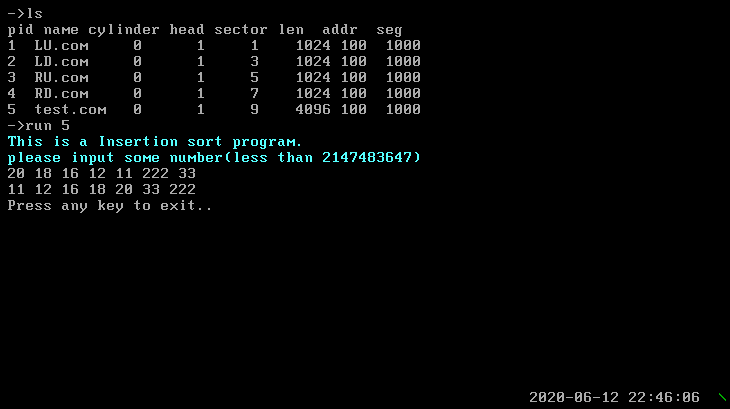
\includegraphics[width=0.8\linewidth]{test.png}
  \caption{test.com}
  \label{fig:test.com}
\end{figure}
图 \ref{fig:test.com}是输入一串数字后,按下回车的结果

之前实验的所有特性在此次实验中都保留(除了Ouch),和之前的实验一样。因此不再做其他的演示。具体的特性可以看录制好的OSdemo.mkv

\section{总结与讨论}

% 特色、问题、教训、改进、收获


\subsection{特色,不足与改进}

本次实验实现了系统调用后,加上执行程序的风格参照dos,不需要约定返回方式,已经可以将用户编写程序的过程与内核完全解耦。原来的特性也完全保留,因此编写程序后,只需要修改用户程序表并将程序放入镜像即可直接使用操作系统加载。
用户程序提供的库函数非常丰富,除了常见的字符串操作和IO外,可以打印彩色的字符串,完成数字字符串的转换等。
不足之处有三点,
\begin{enumerate}
  \item 内核的安全性不足,按照目前的方法,如果将用户程序返回地址放在内核中,下次实现多进程时会因为栈的位置不一致无法从用户程序正常返回,因此内核的许多信息都使用了用户程序的栈存放。
  \item 用户的汇编程序中部分段寄存器的值与内核相关。
  \item 时钟中断和软中断没有使用同一个寄存器映像保存现场,造成代码的冗余,原因在问题部分会解释。
\end{enumerate}


\subsection{收获}

本次实验中,我对软中断和时钟中断有了更深入的了解,掌握了对dos执行程序的过程。在编写和调试保护现场恢复现场的代码时,汇编能力和调试能力有较大的提高。
在编译自己写的c代码时,makefile的编写也更加熟练\cite{makefile}。同时,在本报告的编写过程中,我也练习了利用 \LaTeX 编写文档的能力。\cite{lamport94, cite}

\subsection{遇到的问题}
这次遇到的问题数量不多,但是较上次更为复杂。主要有三点:
\subsubsection{栈不平衡问题}
由于使用了c和汇编的混合编程,而且经常出现汇编调用c函数的情况,在完成与c语言相关的工作时,必须一切都以双字为单位,比如retf和call dword,而汇编则都以字为单位,一旦有不一致,就会出现栈不平衡,在Bochs中会出现“WARNING: HLT instruction with IF=0!”的问题,
这个问题查资料时是不会找到和栈平衡相关的资料的。
\subsubsection{标号问题}
实现系统调用时,我发现在数据区定义时如果把标号声明成双字节,那么在生成的二进制文件中会找不到这个声明的数据。但是声明成双字后就正常。调试的时候用Bochs查看内存发现居然不存在,而且不断修改声明的方式位置,都未能解决问题,除了声明成双字。
原因未知。
\subsubsection{键盘中断导致的死机}
使用了离开程序的中断后,我发现用户com程序一旦触发键盘中断Bochs就会出现int13\_diskette: unsupported AH=10,之后再也无法响应键盘,去掉ouch程序后正常,我认为是嵌套中断导致的问题。
\subsubsection{软中断嵌套时钟中断}
这个问题花费了我数天时间来解决,即便询问了同学和老师,但是目前只有我遇到这个问题。因为我使用cli后认为软中断不会被打断所以我一直认为是restart和save导致的。问题发生在我将restart和save同时放入软中断过程和时钟中断过程中。用户程序一旦运行就会死机。
而在内核中,即便时钟中断依然进行,但是没有任何问题。我再一开始忽视了这个现象,而一直在寻找restart和save的错误。实际上,只有同时时钟中断和软中断同时存在才会出现问题。而在我调试的过程中,我发现restart执行后,iret根本无法返回,
会进入bios程序的死循环,老师的解释是当前的寄存器信息与进入时的不一致,但是因为我时钟中断也执行了cli,所以我以为是restart和save的问题,然而去掉软中断的restart和save之后,调试比较前后寄存器,并没有发现问题。并且在restart返回前,
查看栈里的值,都是非常大的数字(比如fe00),我猜测是bios的原因,认为是触发了某个中断,而且我发现restart时,本地的寄存器映像已经被修改了。并且我在调试时发现如果一直单步执行,程序时没有错误的。
但是一旦使用next,或者continue,就会出现restart时寄存器映像被修改的问题,在同学的建议下,我在restart的执行前一句,加上了时钟中断的断点,并使用next,发现果然进入了时钟中断。并且我还发现,时钟中断的cli处即使设置断点也不会触发,
我猜想是因为根本没有执行。这个问题目前并没有解决,但是代码稍作修改,为时钟中断单独分配一个寄存器映像就不影响实验了。
\subsection{感想}
此次实验既使用了c语言,又使用了汇编,而且完成的工作都比较精细,由于需要不断的调试,我深刻体会到了自动化部署和调试工具的重要性。以及原理和实践之间的差距。这次实验即便花了这么久的时间,仍然是享受到之前实验的便利的,
比如提前设计好的shell的用户程序加载,比如大量的库函数。所以每次实验还是要适当增加内容,减少以后的负担。

\begin{thebibliography}{99}
  
  \bibitem{gityuan2016}
  Gityuan,
  \textit{Linux系统调用(syscall)原理}
  \url{http://gityuan.com/2016/05/21/syscall/}
  2016., \\
  \bibitem{wiki:Interrupt}
  Wikipedia,
  \textit{{Interrupt} --- {W}ikipedia{,} The Free Encyclopedia}
  \url{http://en.wikipedia.org/w/index.php?title=Interrupt&oldid=960304240}
  2020., \\
  \bibitem{csdn2010}
  CSDN,
  \textit{中断 INT 20H}
  \url{https://blog.csdn.net/heavengl/article/details/6035824}
  2010., \\
  \bibitem{makefile}
  how-to-write-makefile,
  \textit{跟我一起写Makefile}
  \url{https://seisman.github.io/how-to-write-makefile/index.html}
  陈皓,
  2020., \\
	\bibitem{lamport94}
  Leslie Lamport,
  \textit{\LaTeX: a document preparation system},
  Addison Wesley, Massachusetts,
  2nd edition,
  1994.   \\
  \bibitem{cite}
  Contributors to Wikibooks,
  \textit{LaTeX Bibliography Management.}
  Wikibooks,
  2019., \\
  en.wikibooks.org/wiki/LaTeX/Bibliography\_Management.
\end{thebibliography}
 
%----------------------------------------------------------------------------------------

\end{document}